\begin{figure}
	\centering
	\footnotesize
	\begin{tabular}{p{3.7cm}p{3.7cm}}
		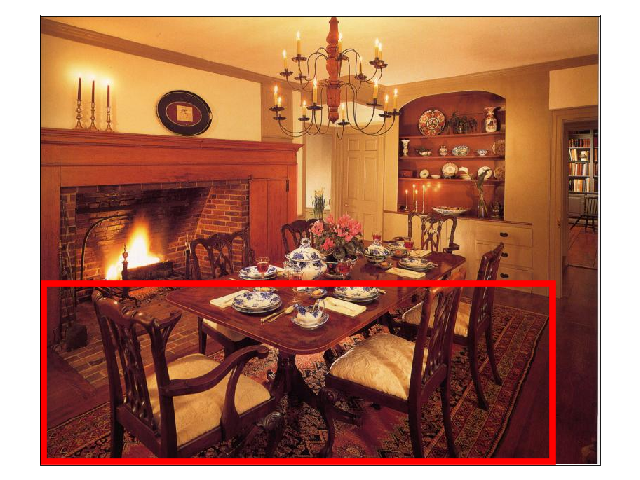
\includegraphics[scale=.2]{images/556_1063956_seed_ambiguous.png} &
		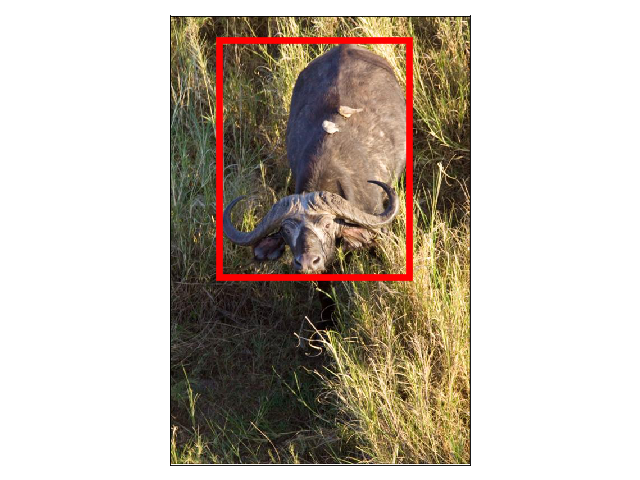
\includegraphics[scale=.2]{images/2657_1069343_singleton_obj.png} 
		\\
		Entry-level: rug (21) &  animal (9)\\
		\midrule
		Same-object: carpet (4, 0.7) &  yak (3,0.8), buffalo (2,0.7) \\
		Error-box: chair (5, 0.5), floor (3, 0.5) & \\
		Error-visual:  & cow (6,0.5), ram (3,0.7), bull (2,0.7)\\
		\midrule
		FRCNN$_{\text{VG1600}}$: floor & animal\\
		FRCNN$_{\text{VG1600--VGMN}}$: rug & cow \\
	\end{tabular}
	\caption{Annotations, verification and predictions for 2 objects: name (number of annotations, adequacy rating)}
	\label{fig:mistakes}
\end{figure}

\begin{table*}[t]
	\centering
	\small
	\begin{tabular}{ll||c|cccc|c}
		\toprule
		&  & Hit & \multicolumn{4}{c|}{Human-like} & Off \\
		Model &  GT &  & SameObject &  OtherObject &  Low Count &  Related &   \\
		\midrule
		FRCNN--VG1600&VG &         74.8 &                13.7 &                  2.9 &              2.4 &              1.7 &          4.5 \\
		FRCNN--MN442&VG &         71.1 &                13.6 &                  3.4 &              2.0 &              2.6 &          7.4 \\
		\midrule
		FRCNN--VG1600--VGMN&MN &         80.7 &                 9.0 &                  2.0 &              1.8 &              3.4 &          3.3 \\
		\midrule
		ResNet101--VGMN&VG &         62.8 &                11.6 &                  2.1 &              3.2 &             10.3 &         10.1 \\
		ResNet101--MN442&VG &         63.8 &                11.9 &                  2.4 &              3.3 &              8.8 &          9.9 \\
		ResNet101--VGMN&MN &         68.7 &                 9.9 &                  3.0 &              2.5 &              7.7 &          8.2 \\
		ResNet101--MN442&MN &         69.7 &                 9.9 &                  3.2 &              2.7 &              7.0 &          7.6 \\	
		\bottomrule
	\end{tabular}
	\caption{Model results for different categories of errors. \label{tab:humanlike}}
\end{table*}

\begin{table*}[t]
	\centering
	\small
	\begin{tabular}{ll|c@{~}c@{~}c@{~}c}
		\toprule
		{Model} &  GT & visual &  linguistic &  box &  other \\
		\midrule
		FRCNN--VG1600 & VG &             4.3 &                 0.0 &                  95.7 &            0.0 \\
		FRCNN--MN442 & VG &             3.4 &                 0.0 &                  96.6 &            0.0 \\
		\midrule
		FRCNN--VG1600--VGMN & MN &             6.7 &                 0.0 &                  93.3 &            0.0 \\
		\midrule
		ResNet101--VGMN & VG &             5.6 &                 0.0 &                  94.4 &            0.0 \\
		ResNet101--MN442 & VG &             4.8 &                 0.0 &                  95.2 &            0.0 \\
		ResNet101--VGMN & MN &             3.1 &                 0.0 &                  96.9 &            0.0 \\
		ResNet101--MN442 & MN &             3.0 &                 0.0 &                  97.0 &            0.0 \\
		\bottomrule
	\end{tabular}
	\caption{Break-down of the instances (in \%) for which the models predicted an \textit{inadequate} name according to the type of inadequacy.  \label{tab:exp_inadequacy}}
\end{table*}


The previous Section \ref{sec:experiments} looked at the performance of the different naming models using vanilla evaluation methods like accuracy.
This way of evaluating object naming is unsatisfactory: the ManyNames data, and also our verification data, clearly shows that human annotators often agree on a certain entry-level name with other names might be adequate too.\cs{XX}
In the following, we show how our verification data can be used to gain more detailed insights into the way different naming models calibrate their decisions and reflect human-like naming behavior.



\paragraph{Error Categories} We categorize model predictions into the following types (also see Figure~\ref{fig:mistakes} for examples):\\
Hit: the entry-level name\\
Off: a non-sensical name (none of the others). \\
Human-like mishits:
\begin{itemize}
\item \sameobject: an alternative name for the object (see Section~\ref{sect:mn_verification}), or a synonym or a hypernym (\name{house/building})
\item OtherObject: a name produced by annotators, but not an alternative of the entry-level name  
\item LowCount: a name produced by only one annotator
\item Related: a hyponym or co-hyponym of the entry-level (\textit{jacket/shirt})
\item Incorrect-off: a non-sensical name (none of the above)
\end{itemize}
We use WordNet for determining whether two names are semantically related   \newcite{fellbaum1998wordnet}. 

\subsection{How Human-Like are Model Predictions and Errors?}

Table \ref{tab:humanlike} shows the breakdown of the model results for the error categories explained above. An important general trend is that the proportion of human-like error seems to be surprisingly constant across all models. \sz{why??}
Both object detection models essentially achieve the same portion of valid predictions. Thus, the main difference of FRCNN$_{\text{MN442}}$ to  FRCNN$_{\text{VG1600}}$ is that the former makes more nonsensical errors (column off), which might be an effect of the reduction in training data.
Importantly, the transferred classification model FRCNN$_{\text{VG1600--VGMN}}$ achieves more hits but less valid predictions, and also less nonsensical errors as compared to FRCNN$_{\text{VG1600}}$.
This suggests that the transfer learning approach is most effective when the object detection model achieves a valid prediction, which is then calibrated to a perfect hit (it predicts the entry-level) by the fine-tuned classification model.
The proportion of instances for which the ResNet models predict a `related'' category is high, which suggests that they tend to confuse semantically similar names to a valid name, that are, however, not valid. 

\iffalse
\begin{table*}[t]
\centering
	\small
\begin{tabular}{ll||rr|rrr}
\toprule
&  & \multicolumn{2}{c|}{Correct} & \multicolumn{3}{c}{Incorrect}\\
                         model &  gt &  hit &  valid &  human-like &  related &  off \\
\midrule
       FRCNN$_{\text{VG1600}}$ &  VG & 74.8 &     13.7 &         5.3 &      1.7 &    4.5 \\
        FRCNN$_{\text{MN442}}$ &  VG & 71.1 &     13.6 &         5.3 &      2.6 &    7.4 \\
        \midrule
 FRCNN$_{\text{VG1600--VGMN}}$ &  MN & 80.7 &      9.0 &         3.7 &      3.4 &    3.3 \\
         \midrule
     ResNet101$_{\text{VGMN}}$ &  VG & 62.8 &     11.6 &         5.2 &     10.3 &   10.1 \\
         ResNet101$_{\text{MN442}}$ &  VG & 63.8 &     11.9 &         5.7 &      8.8 &    9.9 \\
     ResNet101$_{\text{VGMN}}$ &  MN & 68.7 &      9.9 &         5.5 &      7.7 &    8.2 \\
    ResNet101$_{\text{MN442}}$ &  MN & 69.7 &      9.9 &         5.9 &      7.0 &    7.6 \\
\bottomrule
\end{tabular}

\caption{Model results for different categories of errors} \label{tab:humanlike}
\end{table*}
\fi


\paragraph{Why May Models Predict Inadequate Names?}
In Table~\ref{tab:exp_inadequacy} we focus on the predicted names that are in \mn for the corresponding objects, but judged as inadequate (i.e.,~adequacy score$<0.5$). 
Most of the inadequate object name predictions are related to an inaccurate bounding box. 
The overall best FRCNN$_{\text{VG1600--VGMN}}$ model has the smallest proportion of box errors, and hence, the least \textit{visual} (i.e.,~the object is difficult to interpret) inadequate name predictions. 
\iffalse
\cs{remove next couple of sentences? it's very assumptive}
This may be due to it using features pre-trained towards object detection (i.e.,~localization), but then being optimized towards \mn entry-level names. 
And the ResNet101-based models, which use features that were pre-trained towards image classification (i.e.,~categorizing the salient object in an image (region)), make slightly more visual errors when being optimized on \vg ground truth labels than their \mn ground truth counterparts. 
\fi

None of the models predicted an inadequate name that was a linguistic, or any other error. 
The results show that the models make similar mistakes to humans (problems in identifying or recognizing the target object) when being faced with data that was collected with a task setup that approximates human behavior, such as \mn, and the limitations in defining and implementing annotation tasks for data collection of this sort. 


\begin{table*}[t]
\centering
	\small
\begin{tabular}{ll|rrr|rrr}
\toprule
&  & \multicolumn{3}{c|}{MN agreement $>$ 0.9} & \multicolumn{3}{c}{MN agreement $\leq$0.9}\\
                         model &  GT &  hit &  human-like &  off &  hit &  human-like &  off \\
\midrule
       FRCNN$_{\text{VG1600}}$ &  VG &   94.8 &           2.6 &      2.6 &   63.6 &          30.9 &      5.5 \\
        FRCNN$_{\text{MN442}}$ &  VG &   89.6 &           4.2 &      6.2 &   60.7 &          31.3 &      8.0 \\
        \midrule
 FRCNN$_{\text{VG1600--VGMN}}$ &  MN &   94.5 &           4.2 &      1.3 &   72.9 &          22.7 &      4.4 \\
 \midrule
     ResNet101$_{\text{VGMN}}$ &  VG &   88.3 &           6.2 &      5.5 &   48.5 &          38.8 &     12.7 \\
     ResNet101$_{\text{VGMN}}$ &  MN &   89.6 &           5.5 &      4.9 &   57.0 &          32.9 &     10.1 \\
    ResNet101$_{\text{MN442}}$ &  MN &   90.1 &           4.9 &      4.9 &   58.2 &          32.8 &      9.0 \\
    ResNet101$_{\text{MN442}}$ &  VG &   88.6 &           5.2 &      6.2 &   49.9 &          38.2 &     12.0 \\
\bottomrule
\end{tabular}
\caption{Break-down of the results (in \%) according to the agreement level of the MN name: Categorization of a predicted name\ $\hat{n}$ into either a \textit{hit}, \textit{human-like} error (less preferred name, synonym, hypernym/hyponym), or \textit{off} \label{tab:exp_errors_agreement}}
\end{table*}

\iffalse
\begin{figure}
	\centering
	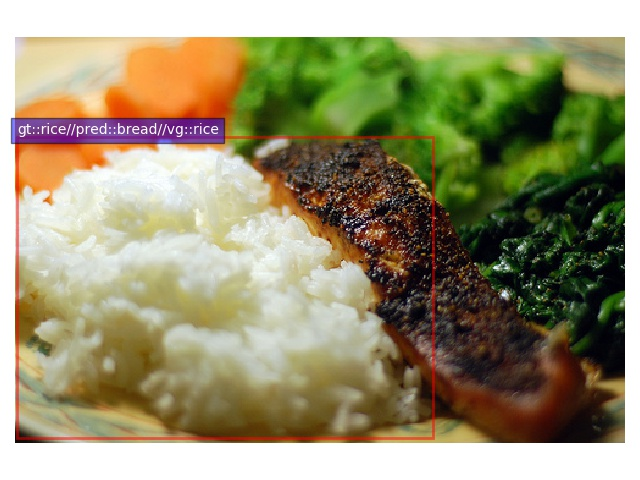
\includegraphics[scale=.2]{images/2323938.jpg}
	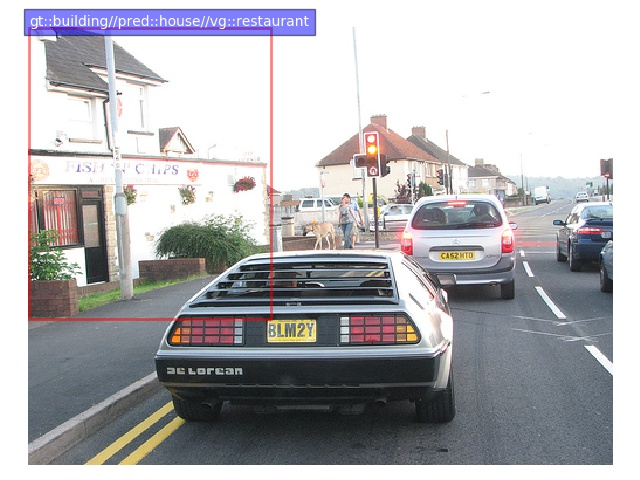
\includegraphics[scale=.2]{images/2322259.jpg}
	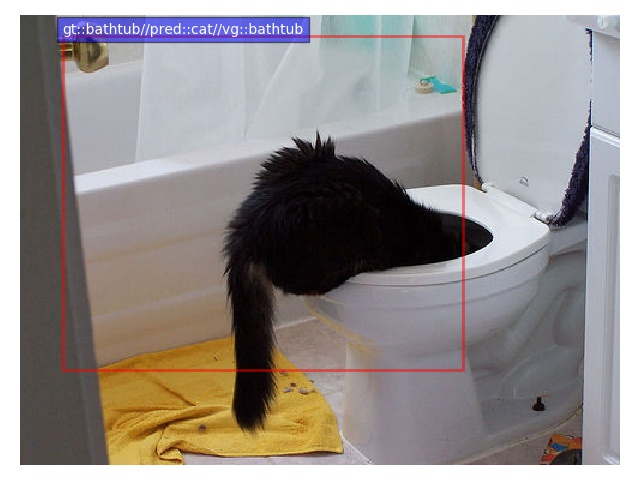
\includegraphics[scale=.2]{images/2371657.jpg}
	
	\caption{TODO: examples resnet mistakes (trained on vg\_manynames, tested on manynames-442)\label{fig:mistakes} \gbt{Will we have space for the figure? (Maybe we should \textit{make} space?) Also, shouldn't we put examples from the most successful model instead?}}
\end{figure}
\fi 



\subsection{How do predictions correlate with human agreement?}

An important observation in Section \ref{sec:manynames} is that even the high number of annotations for an object in ManyNames might not be enough to be fully confident about the entry-level name.
This suggests that there is a certain portion of objects in the dataset that could be difficult to name even for humans, e.g.,~for linguistic reasons (they don't know how to name the object adequately), or whose name depends on the speaker's interpretation of the situation in which the object is shown, such that an agreement on a certain name is difficult to achieve. \sz{is it okay to claim this?}.\cs{how about the way it is now?}
In Table \ref{tab:exp_errors_agreement}, we show the break-down of model predictions and errors for objects with high and low naming agreement in ManyNames, i.e.\ objects where more or less than 90\% of the annotators opted for the entry-level name. 
Here, we find a very clear pattern for all models, namely that the portion of hits is generally high when human agreement is also high.
Note that this even holds for the ResNet-based classifiers that generally achieve less accuracy.
When agreement is lower, all models produce less hits and more valid alternatives. 
This indicates that there is indeed a certain similarity between what is difficult for humans and models.
Interestingly, also the portion of incorrect predictions is substantially higher when the agreement is lower. \sz{why???}


%\cs{TODO::}
%Categorization of "errors" ():
%\begin{enumerate}
%	\item Clear mistake \\
%	e.g.,\ rice vs. bread
%	\item Alternative name\\
%	e.g.,\ building vs. house
%	\item Alternative object \cs{(other cluster from verif data)}
%	\item Synonym\\
%	e.g.,\ plane vs. airplane
%	\item Semantically related\\
%	e.g.,\  motorcycle vs. scooter
%\end{enumerate}










%%% Local Variables:
%%% mode: latex
%%% TeX-master: "acl2020_main"
%%% End:
